
%Volume: maximaal aantal pagina van inleiding t/m literatuur, maximaal  35 bladzijden (excl.bijlagen).
\documentclass[11pt]{report}
\usepackage[a4 paper, headheight=1pt, headsep=1pt] {geometry}
\usepackage{titlesec}
\titleformat{\chapter}[display]   
{\normalfont\huge\bfseries}{\chaptertitlename\ \thechapter}{8pt}{\huge}   
\titlespacing*{\chapter}{0pt}{-65pt}{8pt}
\titlespacing*{\section}{0pt}{5pt}{1pt}
\setlength{\parindent}{0pt}
\setlength{\parskip}{5pt plus 2pt minus 1pt}
\setlength{\textheight}{680pt}
\setlength{\headsep}{0pt}
%\usepackage{showframe}
\usepackage{graphicx}
\usepackage[usenames,dvipsnames]{color}
%\usepackage{picins}
\footskip = 20pt 
\usepackage[nodayofweek]{datetime}
\usepackage{tikz}
\usepackage{todonotes}
\usepackage{float}

\usepackage{pdfpages}
\usepackage{siunitx}
\usepackage{multirow,colortbl,array}
\usepackage[HTML]{xcolor}

\usepackage{wrapfig}

\begin{document}
\begin{titlepage}
	\begin{center}
	\vspace*{0\textheight}
	{\scshape\LARGE Utrecht University \par} 
	\vspace{1cm} 
	\line(4,0){300}
	\vspace{0.5cm} \\
	{\Large \bfseries Local characteristics of two Svalbard glaciers\\}
	\vspace{0.5cm}
	\line(4,0){300} \\

	\vspace{2.5cm}
	\begin{minipage}[t]{0.4\textwidth}
	\begin{flushleft} \large
	\emph{Authors:}\\
	{Isolde Glissenaar}\\
	{Daphne van Zanten} \\
	\end{flushleft}
	\end{minipage} %No ENTER BECAUSE!
	\begin{minipage}[t]{0.4\textwidth}
	\begin{flushright} \large
	\emph{Supervisor:} \\
	{Dr. C.H. Tijm-Reijmer}\\
	\end{flushright}
	\end{minipage}\\[0.4cm]

	\vspace{7.5cm}
	\large \textit{}\\[1cm]

	{\large {\today}\\[2cm] % Date

	\noindent
	
\includegraphics[scale=1, width=0.4\textwidth]{UU-logo.jpg}
	\hspace{0.2\textwidth}
	
\includegraphics[scale=1, width=0.22\textwidth]{imau.png}}
	\end{center}
\end{titlepage}

\newpage
\tableofcontents

\chapter{Introduction}\label{sec:intro}
\pagenumbering{arabic}
\setcounter{page}{3}
%\todo{In report: \\
%- General description experiment and conditions\\
%– General description of the dataset and data handling\\
%– Detailed analyses of chosen subject\\
%+- 15 pages}

Around 1595, a Dutch man called Willem Barentsz went on expedition to search for a North East Passage when he discovered Svalbard \cite{sval}. To imagine this situation, a painting of his ship is made by Arnold de Lange and shown in figure \ref{fig:wbs}. From this moment on, Dutch people invested in research on Svalbard's climate and ecology. Around 2010, the interest in research on the eastern side of the island Spitsbergen increased. However, there is a small amount of data from this part of the archipelago. To investigate the present situation and organize a new expedition to this part of the archipelago, SEES (Netherlands Scientific Expedition Edge\o ya Spitsbergen) has been established, which is still active nowadays \cite{sees}. SEES organized an expedition in august 2015 during which an Automatic Weather Station was installed on the Ulvebreen.

\begin{figure}[h]
\includegraphics[scale=1, width=0.5\textwidth]{wbs.jpg}
\centering{}
\caption{Ship of Willem Barentsz at the discovery of Svalbard, made by Maritim painter Arnold de Lange}
\label{fig:wbs}
\end{figure}

In our project, we retrieved measurement data from three weather stations in Svalbard. Two are located on glaciers (Nordenski\H{o}ldbreen and Ulvebreen) and one on land (Svalbard Lufthavn). In this study, measurement data from the three locations on Svalbard is used to answer the following question:

\textbf{\textit{How can the local conditions on two Svalbard glaciers be explained?}}

To investigate this, sub-questions arise:
\textit{What are the characteristics of the Nordenski\H{o}ldbreen and the Ulvebreen?} and \textit{What are the differences between the two glaciers?}

Explained in chapter \ref{sec:method} is the origin of the measurements and the data handling methods. Chapter \ref{sec:results} contains results of this research, obtained by comparing data. In chapter \ref{sec:discussion} results are discussed and compared with the hypothesis. In chapter \ref{sec:conclusion}, a conclusion is presented.

\newpage

\chapter{Method}\label{sec:method}

To investigate the local characteristics of two glaciers on Svalbard, the location of the glaciers are described in section \ref{sec:loc}. On those glaciers, instruments are installed to measure different variables, which are described in section \ref{sec:instr}. Finally, the data handling is discussed in section \ref{sec:datah} and the main used calculations are explained in section \ref{sec:calc}.

%\textcolor{red}{location of measurements, instruments, data handling (on making the daily averages and handling the data gaps.)} are investigated. 

\section{Location} \label{sec:loc}
This study discusses data from weather stations situated on Svalbard, which is a Norwegian archipelago in the Arctic Ocean, north of the European mainland. The island group ranges from 74$^\circ$N to 81$^\circ$N in latitude. The archipelago features an Arctic climate, although with higher temperatures than other areas on the same latitude. The northernmost branch of the relatively warm North Atlantic Current, the West Spitsbergen Current, as shown in figure \ref{fig:current}, moderates the temperature on the western side of the island. The East Spitsbergen Current brings colder water from higher latitudes to the eastern side of the archipelago. The mean temperatures range from $\SI{-16}{^\circ C}$ in February to $\SI{6}{^\circ C}$ in July \cite{1} at Svalbard Lufthavn, in the middle of the main island Spitsbergen. The mean yearly precipitation at Svalbard Lufthavn is 190 mm. 

\begin{figure}[h]
\includegraphics[scale=1, width=0.5\textwidth]{currents_svalbard.jpg}
\centering{}
\caption{Map of Svalbard showing key features and major ocean currents \cite{2}.}
\label{fig:current}
\end{figure}

All three measurement locations are situated on the largest island, called Spitsbergen. Data is used from two weather stations from the Institute for Marine and Atmospheric research Utrecht (IMAU) located on two glaciers, and data from an operational station from the Norwegian Meteorological Institute, as shown in figure \ref{fig:locations}.

\begin{figure}[h]
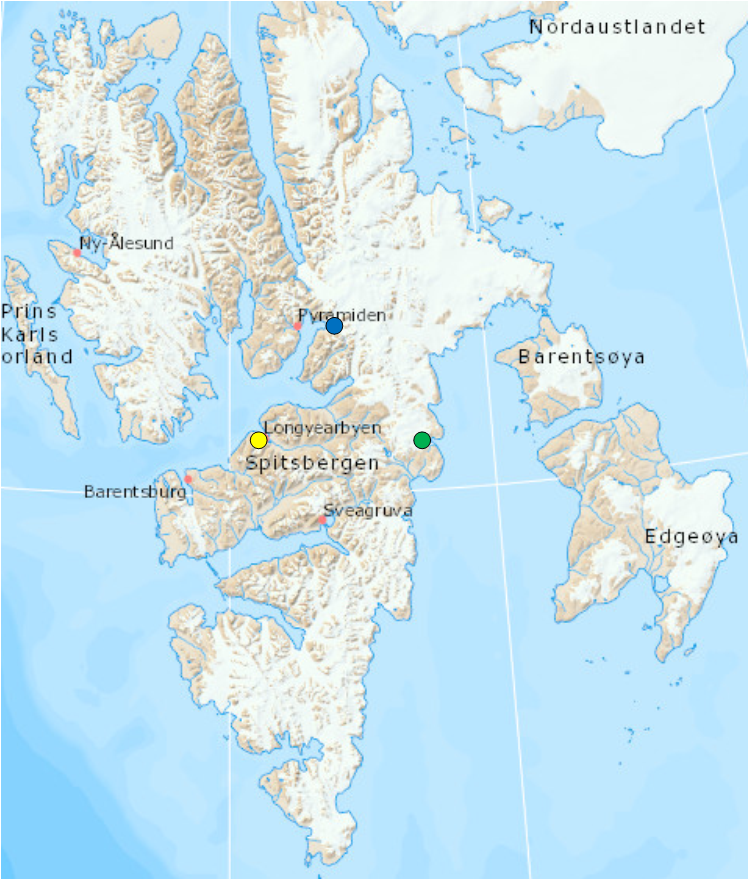
\includegraphics[scale=1, width=0.5\textwidth]{svalbard_locations.png}
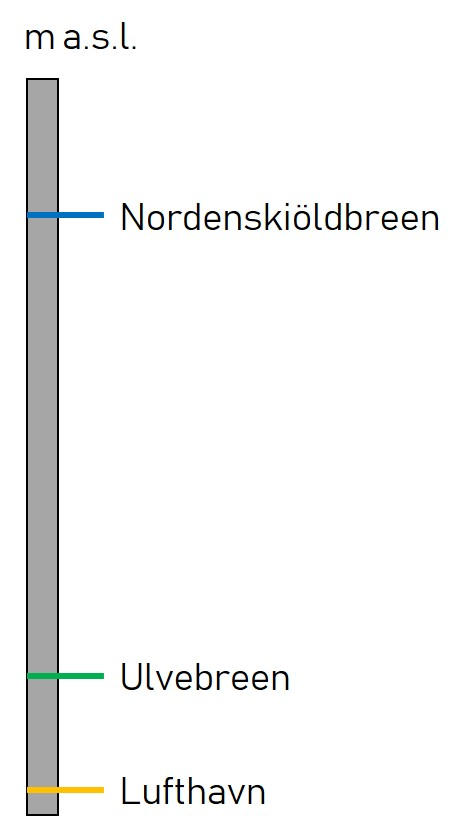
\includegraphics[scale=1, width=0.33\textwidth]{height.jpg}
\centering{}
\caption{Left: Map \cite{NPI} of Svalbard showing the locations of the weather stations. Blue: Nordenski\H{o}ldbreen, green: Ulvebreen, yellow: Svalbard Lufthavn. Right: Schematic picture of differences in height}
\label{fig:locations}
\end{figure}

The weather stations are situated on the Nordenski\H{o}ldbreen and the Ulvebreen. The Nordenski\H{o}ldbreen is a marine-terminating glacier, terminating in Adolfsbukta, which is a branch of Billefjorden. The glacier is situated roughly in the middle of the island Spitsbergen. The glacier is $\SI{25}{km}$ long, $\SI{11}{km}$ wide and located 529 meters above sea level (m a.s.l.). It originates from Lomonosovfonna and flows in southwesterly direction, as shown in figure \ref{fig:norden}. The Ulvebreen is also a marine-terminating glacier. This glacier is a tributary to Nordmannsfonna and terminates in Dunérbukta, at the east of Spitsbergen. The Ulvebreen is $\SI{9}{km}$ long, $\SI{2.5}{km}$ wide and located at 140 m a.s.l., which is a difference of $\SI{389}{m}$ compared to the Nordenski\H{o}ldbreen. It flows in southeasterly direction as visible in figure \ref{fig:ulve}. The third measurement location is an operational station at Svalbard Lufthavn, close to the largest settlement on Svalbard: Longyearbyen. This operational station is run by the Norwegian Meteorological Institute. Svalbard Lufthavn is located at Adventfjorden, which debouches into Isfjorden. It has a height of 28 m a.s.l., which is a difference of $\SI{501}{m}$ with the Nordenski\H{o}ldbreen and $\SI{112}{m}$ with the Ulvebreen, also schematically drawn in figure \ref{fig:locations}. The distance between the Lufthavn and the Nordenski\H{o}ldbreen is around $\SI{60}{m}$, while the distance between Lufthavn and the Ulvebreen is approximately $\SI{70}{km}$. The distance between the Nordenski\H{o}ldbreen and the Ulvebreen is roughly $\SI{65}{km}$. 

\begin{figure}[h]
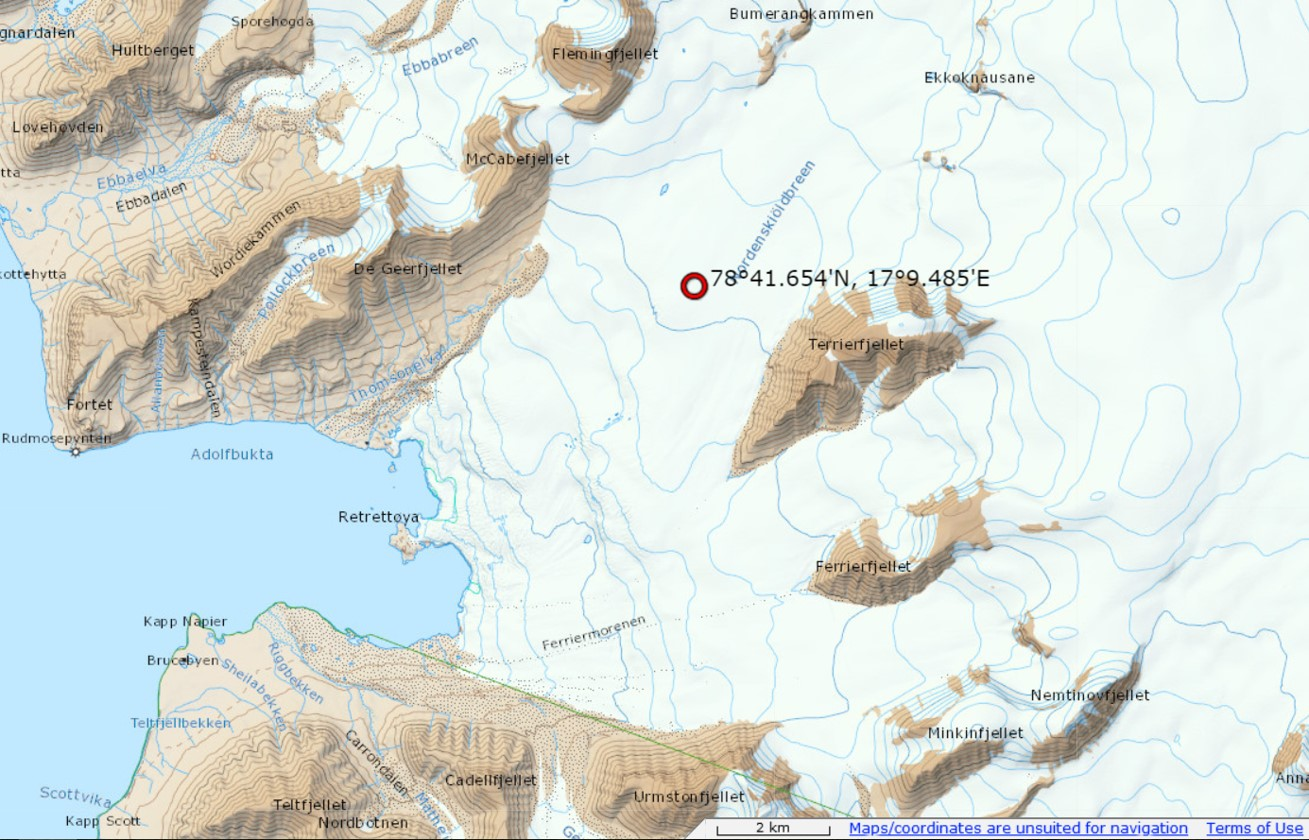
\includegraphics[scale=1, width=0.45\textwidth]{nskimap.jpg}
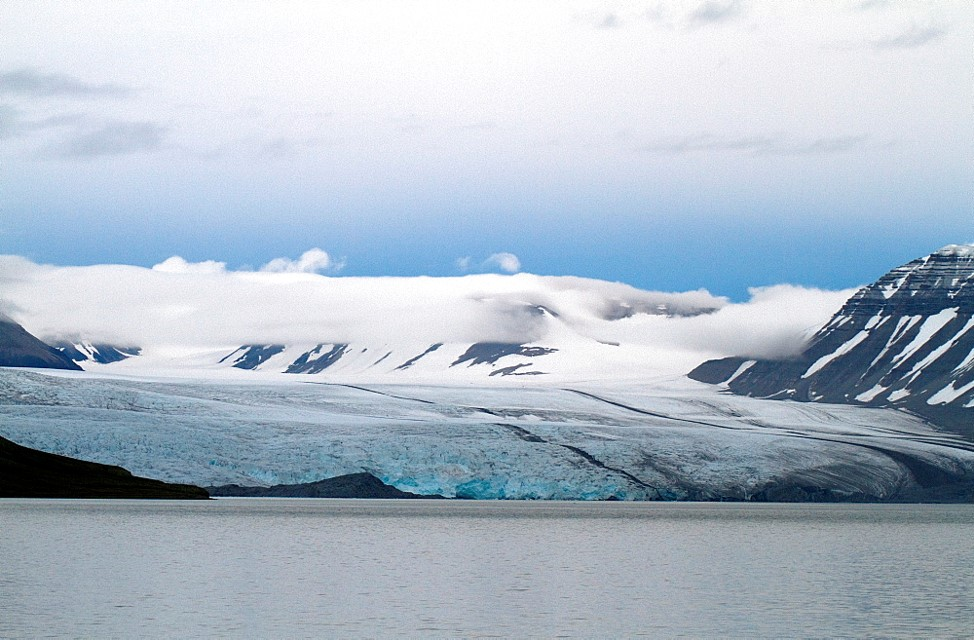
\includegraphics[scale=1, width=0.45\textwidth]{view1.jpg}
\centering{}
\caption{Left: Map \cite{NPI} showing the Nordenski\H{o}ldbreen and the location of the weather station (toposvalbard). Right: A picture of the terminus of the Nordenski\H{o}ldbreen in Adolfsbukta.}
\label{fig:norden}
\end{figure}

\begin{figure}[h]
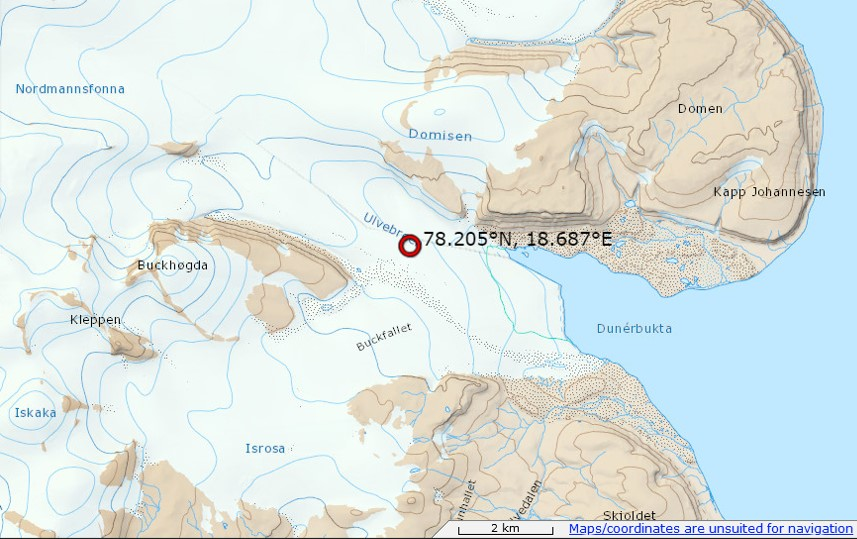
\includegraphics[scale=1, width=0.45\textwidth]{ulvemap.jpg}
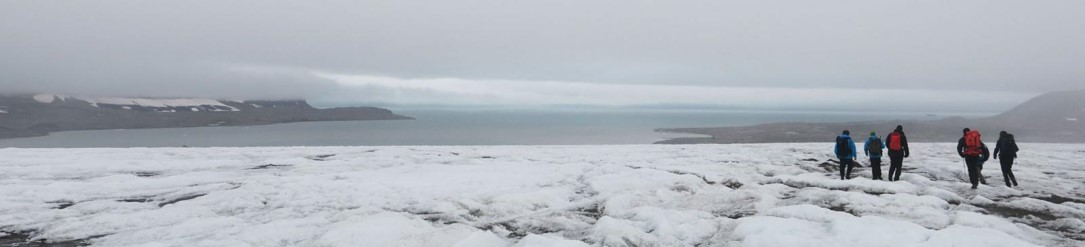
\includegraphics[scale=1, width=0.45\textwidth]{view2.jpg}
\centering{}
\caption{Left: Map \cite{NPI} showing the Ulvebreen and the location of the weather station (toposvalbard). Right: A picture made on top of the Ulvebreen (IMAU).}
\label{fig:ulve}
\end{figure}

\newpage
\section{Instruments}\label{sec:instr}
Measurement data used for this study is mainly retrieved from two Automatic Weather Stations (AWS) on glaciers. The AWS on the Nordenski\H{o}ldbreen is depicted in figure \ref{fig:instrn} and the AWS on the Ulvebreen in figure \ref{fig:instru}.

\begin{figure}[h]
\raggedright
\begin{minipage}{0.5\textwidth}
\centering{}
    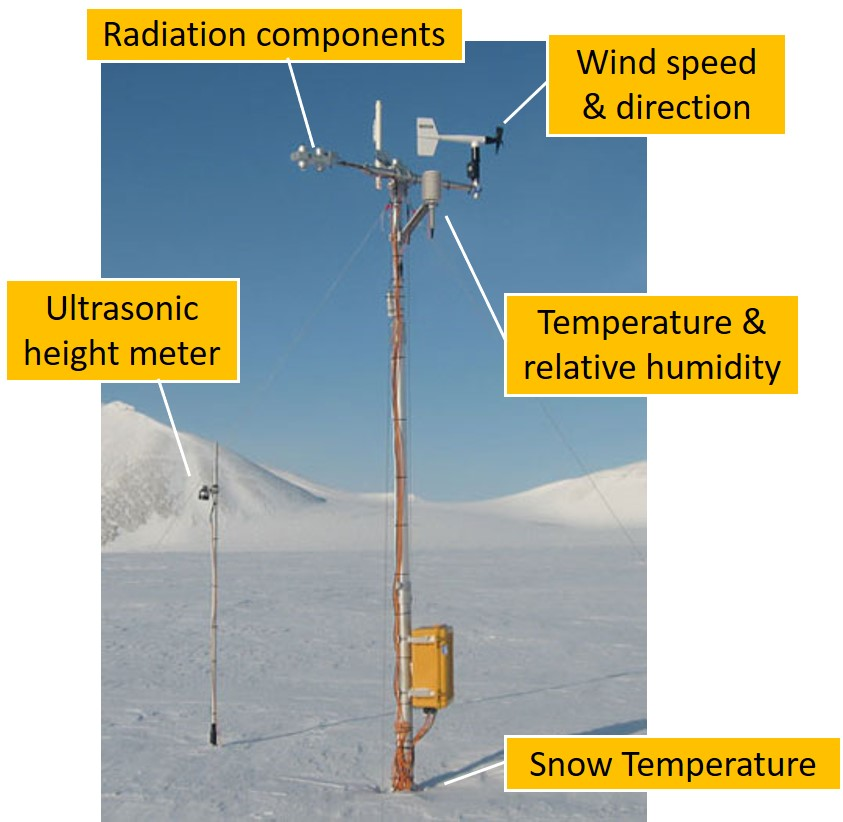
\includegraphics[width=0.9\textwidth]{nski1.jpg}
    \caption{AWS Nordenski\H{o}ldbreen \cite{uuproj}}
    \label{fig:instrn}
\end{minipage}%
\begin{minipage}{0.5\textwidth}
\centering{}
    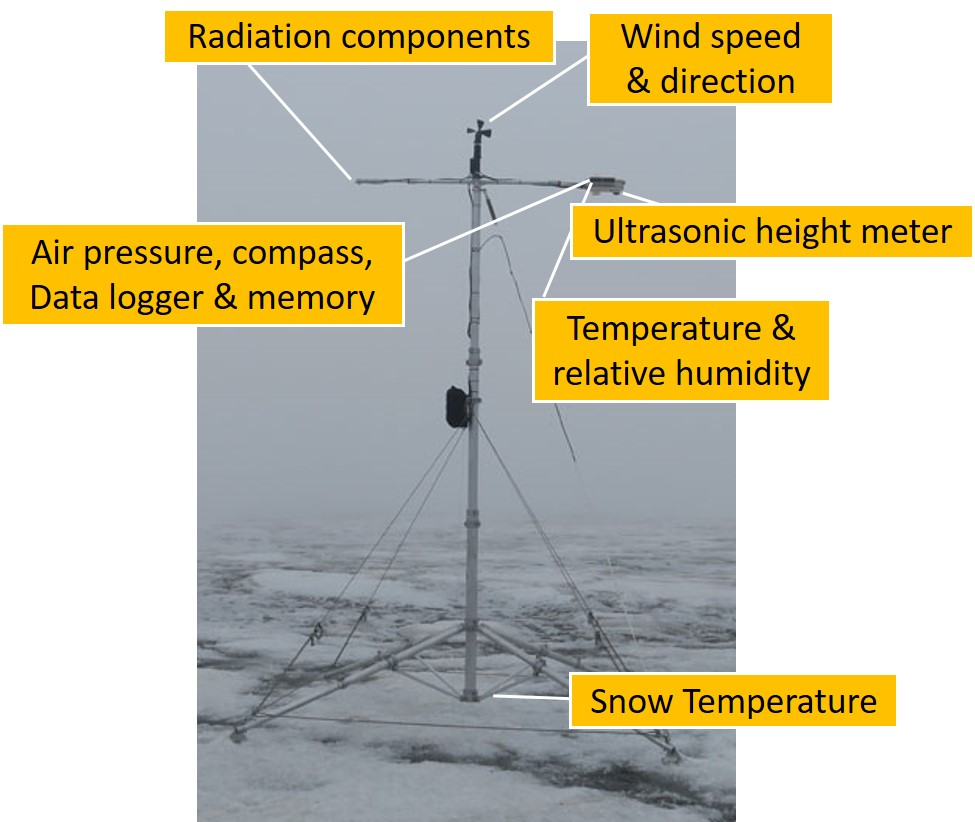
\includegraphics[width=1.05\textwidth]{ulve1.jpg}
    \caption{AWS Ulvebreen \cite{uuproj}}
    \label{fig:instru}
\end{minipage}%
\end{figure}

In figures \ref{fig:instrn} and \ref{fig:instru}, different instruments are visible, where each instrument has his own purpose. Next the different measured variables at the Nordenski\H{o}ldbreen and the Ulvebreen are explained. Finally, the used measurement data of the Lufthavn is described.\\

The AWS on the Nordenski\H{o}ldbreen was operational from March 2009 until December 2016. Within this time, measurements of different variables for timesteps of 30 minutes were saved onto the logger. Unfortunately, because of broken instruments and a location which is hard to reach, there are gaps in the measurement data for the Nordenski\H{o}ldbreen. It should be noted that the AWS on the Nordenski\H{o}ldbreen is drilled into the ice of the glacier, so the height does not change due to the melting of the ice. The weather station uses different instruments. Firstly, the temperature is measured with a thermometer. An anemometer is used to measure the horizontal wind speed and direction. A radiometer with two pyranometers is used to measure the shortwave and longwave radiation for incoming and outgoing directions. A barometer measures the pressure. The snow temperature is measured at 10 different depths. The snow height is measured with an ultrasonic sound meter. An inclinometer is used to measure the tilt.  Finally, the battery is logged as well as the temperature in the logger, to look at the status of the instruments themselves. With all those measurements, the surface temperature is derived from the outgoing longwave radiation. The potential temperature is based on the main hut temperature and pressure. The temperature at 2 meter is based on the main hut temperature and the sonic snow height. The specific humidity is based on the main hut temperature and pressure. \\

The AWS on the Ulvebreen is placed as part of the Netherlands Scientific Expedition Edge$ø$ya Spitsbergen (SEES) in August 2015 \cite{uuproj}. Like at the Nordenski\H{o}ldbreen, every 30 minutes data is saved to a logger and this process is still ongoing (the measuremnts from this station also have some data gaps). The AWS on the Ulvebreen is slightly different compared to the one on the Nordenski\H{o}ldbreen. The AWS on the Ulvebreen is positioned on top of the glacier and is therefor freely to move with the ice. This gives a different result in the snow height measurements. On the Nordenskiöldbreen (where the AWS is drilled into the ice), the snow height measurements give the height of the weather station above the top of the glacier and therefor also increases if the ice melts. On the Ulvebreen however, only the snow melt is recorded with the ultrasonic sensor. However, the AWS on the Ulvebreen also includes an ablation draw wire, which is used to study the ice melt. Figure \ref{fig:ablation} shows a schematic picture of the ablation wire. 

\begin{figure}[h]
\raggedright
\begin{minipage}{0.65\textwidth}
\raggedright
    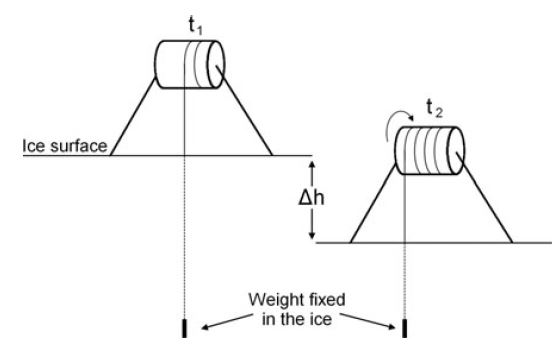
\includegraphics[scale=1, width=1\textwidth]{abliationwire.jpg}	 
    \caption{Ablation Wire \cite{abl}}
    \label{fig:ablation}
\end{minipage}%
\end{figure}

As visible in figure \ref{fig:ablation}, weights are fixed in the ice. A draw wire sensor is placed on top of the ice. This sensor is measuring the height above the fixed weight \cite{abl}. A decrease in height is caused by the ablation of the glacier.

Finally, from the observation station on Svalbard Lufthavn, only data of the wind direction and wind speed, air pressure at station level and air temperature is used to compare this with the two glaciers.

\newpage
\section{Data handling}\label{sec:datah}
As described before, the dataset from the AWS on the Ulvebreen consists of data every 30 minutes from 2015-08-22 to 2018-09-13. The dataset from the Nordenski\H{o}ldbreen AWS also contains 30 minute data from 2009-03-24 to 2016-12-03. Weather data from Svalbard Lufthavn were downloaded from the Norwegian Meteorological Institute \cite{sharkii} and contains 6 hourly data from 0, 6, 12 and 18 UTC. The download consists of data from 2009-03-24 to 2018-09-13, the dates on which also data from the glaciers are available. All three datasets have a few shorter and longer gaps in measurements, caused by the failure of instruments (Ulvebreen and Nordenski\H{o}ldbreen) or too high uncertainty of the measurements (Lufthavn). To study trends in the long time series, daily averages of the data were made. The daily averages were calculated for the Ulvebreen and the Nordenski\H{o}ldbreen if at least 20 datapoints of that day were available. If there were less datapoints available the daily average was possibly not representative and thus assigned a "Not a Number"  (NaN) value. Because for the measurements at Lufthavn there are only measurements a day, the daily average was calculated if at least 3 datapoints were available. 

For the comparison between the three data stations, the data was cut to the period of time where all three stations have measurements, which is from 2015-08-22 to 2016-12-03. This period will from now on be called the data overlap period. Only the daily averages are used if they were calculated for all three stations. If one of them had a NaN value, this day was not used.

\section{Calculations}\label{sec:calc}
To compare temperatures with each other, as discussed in section \ref{sec:T}, a correction for height is applicable. To correct for the difference in height, for all three measurement locations the expected temperature at sea level are calculated by using the lapse rate. A lapse rate of $\SI{-6}{^{\circ}C/km}$ is used, meaning that a location at \SI{1}{km} higher should be $\SI{6}{^{\circ}C}$ colder.\cite{brzblak} Calculating the expected temperature for the Nordenski\H{o}ldbreen at sea level gives:

\begin{equation}
    T_{corrected} = \SI{-7.0}{^\circ C} + \SI{6}{^\circ C/km} \cdot \SI{0.529}{km} = \SI{-3.83}{^\circ C}
    \label{eq:Tatsl}
\end{equation}

The same is done for the other two locations, giving a corrected mean temperature of $\SI{-4.04}{^\circ C}$ for the Ulvebreen and $\SI{-1.95}{^\circ C}$ for the Lufthavn. It can be noted that the mean temperatures corrected to sea level are not equal, so the difference in mean temperature is not only caused by differences in height. 

For a discussion on snow and albedo in section \ref{sec:rad}, the albedo was calculated. This was done for both glaciers by dividing the shortwave incoming radiation with the shortwave outgoing radiation. Because of the fact that there is no incoming shortwave radiation in the polar night in winter, a threshold value for shortwave incoming radiation of $\SI{10}{W/m^2}$ was used. If there was less shortwave incoming radiation, the albedo was NaN. 


\newpage
\chapter{Results}\label{sec:results}
In this chapter, results of the investigation of the data are described in different sections. First, a comparison of the temperature at the weather stations is made, which is described in section \ref{sec:T}. Secondly, the wind directions differ for each glacier, which is in detail described in section \ref{sec:katw}. Finally, the snow height and albedo are investigated and explained in section \ref{sec:rad}.

\section{Temperature} \label{sec:T}
The daily average temperature at a height of two meter is compared for the Lufthavn, Ulvebreen and Nordenski\H{o}ldbreen during the data overlap period (figure \ref{fig:T2m}). From this plot, Nordenski\H{o}ldbreen seems colder than Ulvebreen, while the Lufthaven seems warmer. The mean value for the 2 meter temperature during this period is $\SI{-7.0}{^{\circ}C}$ at the Nordenski\H{o}ldbreen, $\SI{-4.9}{^{\circ}C}$ at the Ulvebreen and $\SI{-2.1}{^{\circ}C}$ at Lufthavn. The main difference between mean temperature is caused by the difference in height of the locations. The Nordenski\H{o}ldbreen is located at 529 meters a.s.l, the Ulvebreen at 140 meters a.s.l. and Svalbard Lufthavn at 28 meters a.s.l., as described in section \ref{sec:loc}. 

\begin{figure}[h]
\centering{}
    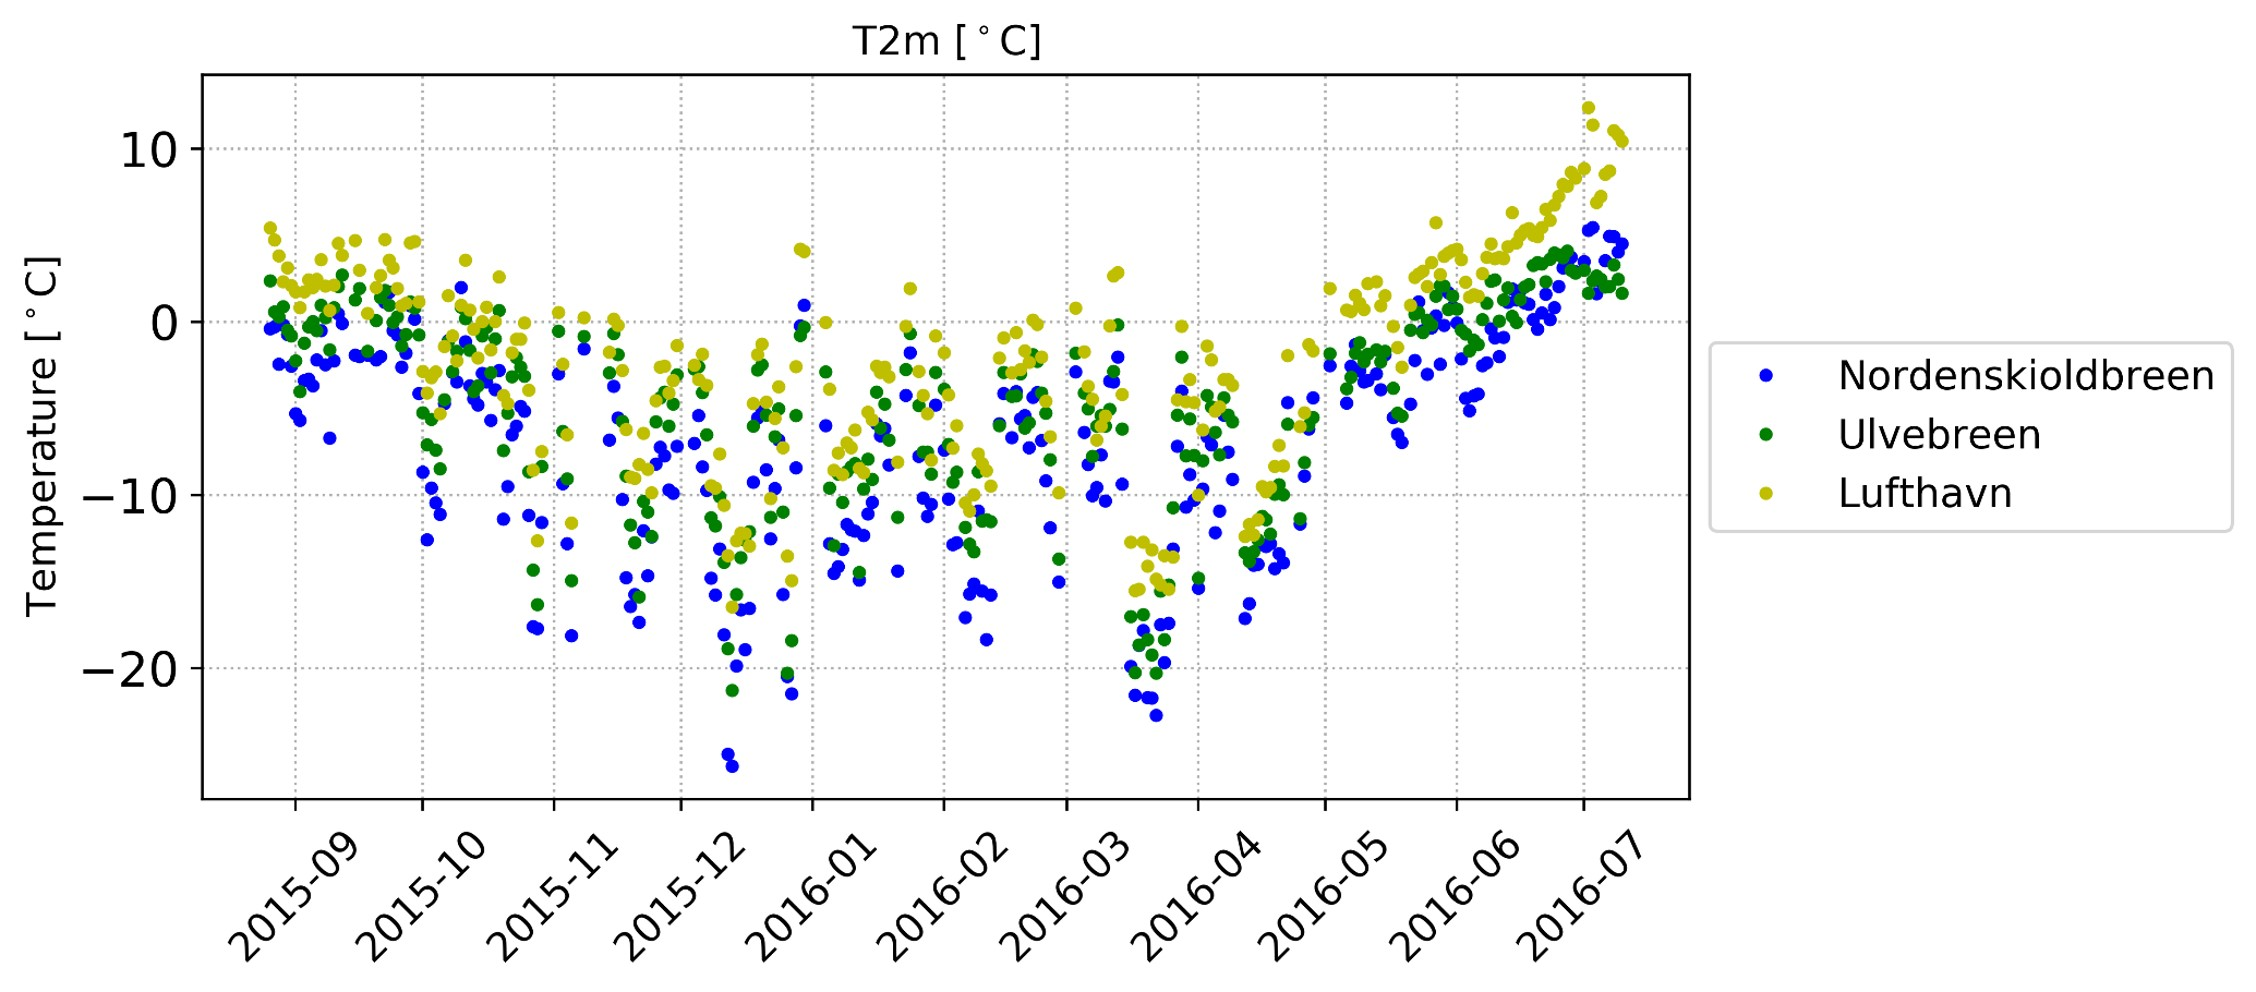
\includegraphics[scale=1, width=1\textwidth]{T2m.jpg}
    \label{fig:T2m}
    \caption{Comparison of temperature at 2 meter height (T2m) for Nordenski\H{o}ldbreen, Ulvebreen and Lufthavn, where colours are corresponding to the legend.}
\end{figure}

The differences in mean temperature after correcting for height by using the lapse rate, explained in section \ref{sec:calc}, are shown in table \ref{tb:avg}. To investigate if the results are significant, a t-test is done. A red cell is corresponding to a significant difference in temperature. 

\begin{table}[h]
\caption{Differences (row minus column) in mean temperature (in degrees Celcius or Kelvin) between locations after correcting for height by the lapse rate. Significance was tested with a T-test, where a red cell is corresponding to a significant value.}
\begin{tabular}{|l|l|l|l|l|}
\hline
\textbf{Location}          & \textbf{Height (m)} & \textbf{Nordenski\H{o}ldbreen}                      & \textbf{Ulvebreen}          & \textbf{Lufthavn}                               \\ \hline
\textbf{Nordenski\H{o}ldbreen} & 529                 & \cellcolor[HTML]{C0C0C0}{\color[HTML]{9B9B9B} } & 0.22                        & \cellcolor[HTML]{FE996B}-1.9                    \\ \hline
\textbf{Ulvebreen}         & 140                 & -0.22                                           & \cellcolor[HTML]{C0C0C0}    & \cellcolor[HTML]{FE996B}-2.1                    \\ \hline
\textbf{Lufthavn}          & 28                  & \cellcolor[HTML]{FE996B}1.9                     & \cellcolor[HTML]{FE996B}2.1 & \cellcolor[HTML]{C0C0C0}{\color[HTML]{9B9B9B} } \\ \hline
\end{tabular}
\label{tb:avg}
\end{table}

As visible in table \ref{tb:avg}, the differences in corrected mean temperature between the two glaciers are not significant, while the difference between the Lufthavn and both glaciers is significant. The causes of this will be discussed in section \ref{sec:Tdisc}. \\

Shown in figure \ref{fig:Tsurf} is a comparison between the surface temperature of both the Nordenski\H{o}ldbreen and the Ulvebreen for the data overlap period. Shown in colour is the date, where red is in summer, blue is in winter and pink in autumn and spring. The surface temperatures of the Nordenski\H{o}ldbreen are lower than those of the Ulvebreen, again due to the height. To correct for this, the lapse rate is added to the data, corresponding to the black line in figure \ref{fig:Tsurf}. To illustrate this: when a temperature of \SI{-10}{^\circ C} is reached at the Ulvebreen, it has to be \SI{-12.3}{^\circ C} at Nordenski\H{o}ldbreen when corrected for height. The remaining difference in surface temperature of the Ulvebreen compared to the Nordenski\H{o}ldbreen is not significant.

\begin{figure}[H]
\centering{}
    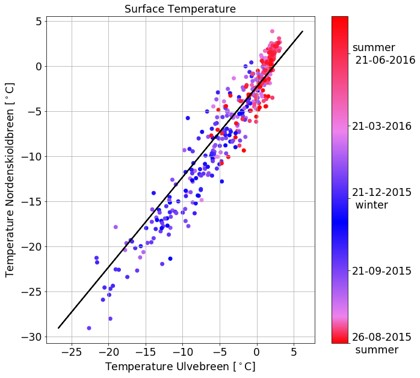
\includegraphics[scale=1, width=0.6\textwidth]{Tsurf.jpg}
    \caption{Comparison of surface temperature of Ulvebreen, visible at the x-axis and the Nordenski\H{o}ldbreen, visible at the y-axis. In colours, the dates are visible from summer 2015 in red below, via winter 2015 in blue, to summer 2016 above, again in red. For explanation of the black line, see main text.}
    \label{fig:Tsurf}
\end{figure}

In the top right of figure \ref{fig:Tsurf} it can be seen that the surface temperature goes above $\SI{0}{^\circ C}$ on both glaciers. This is not expected, because at a value of $\SI{0}{^\circ C}$, the extra energy will be used for ice melt. It can also be seen that the surface temperatures at the Nordenski\H{o}ldbreen rise even more above $\SI{0}{^\circ C}$ than the surface temperatures at the Ulvebreen. The fact that the measurements show a surface temperature above $\SI{0}{^\circ C}$ can be caused by a measurement uncertainty. A possible cause is that in summer, the sensors heat up by the solar radiation. To investigate this hypothesis, the incoming shortwave radiation and wind speed for the Nordenski\H{o}ldbreen are plotted against each other, with the surface temperature in colour, in figure \ref{fig:Thut2}. In this plot all the available data is used, without taking the daily average. 

\newpage
It can be seen that for a high incoming shortwave radiation, the surface temperatures are higher if the wind speed is relatively low. It is thus possible that for high incoming shortwave radiation the sensor, and the few centimeters of air between the surface and the sensor, heats. This will be further discussed in section \ref{sec:Tdisc}.

\begin{figure}[H]
\centering{}
    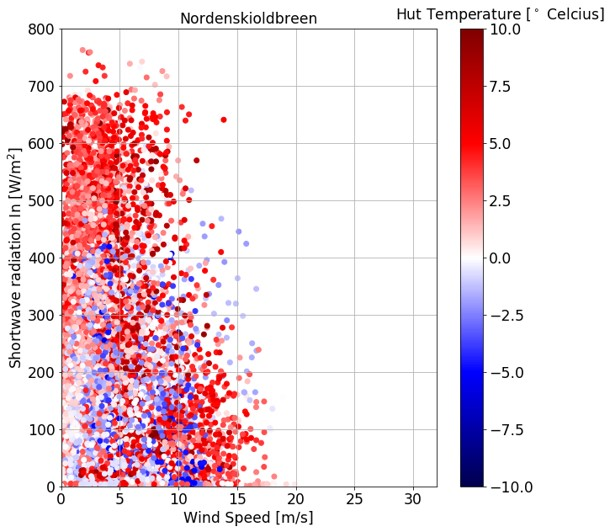
\includegraphics[scale=1, width=0.6\textwidth]{Thut-Sin.jpg}
    \caption{Comparison of the wind speed at the x-axis, the incoming shortwave radiation at the y-axis and the surface temperature corresponding to the colourbar at Nordenski\H{o}ldbreen for all available years between 21 June and 21 September (summer).}
    \label{fig:Thut2}
\end{figure}

\section{Prevailing winds}\label{sec:katw}
Next to the temperatures of the glaciers, differences in wind direction and wind speed are investigated. This is done for both glaciers separately. Results are visible in figure \ref{fig:PR}. Within these plots, clearly visible are the lower values of pressures at higher wind speeds and vice versa. These are caused by large scale weather systems passing over the island. The low pressure systems cause more storms and associated with higher wind speeds. It can also be seen that the wind speeds are higher from some wind directions, for example at the Nordenski\H{o}ldbreen at around 60 degrees and at the Ulvebreen at 250 degrees. To investigate this further, the difference in two meter temperature (T2m) and surface temperature (Tsurf) are plotted in colour instead of the related pressure, which is visible for the Nordenski\H{o}ldbreen in figure \ref{fig:PRnorde} and for the Ulvebreen in figure \ref{fig:PRulve}. 

\begin{figure}[h]
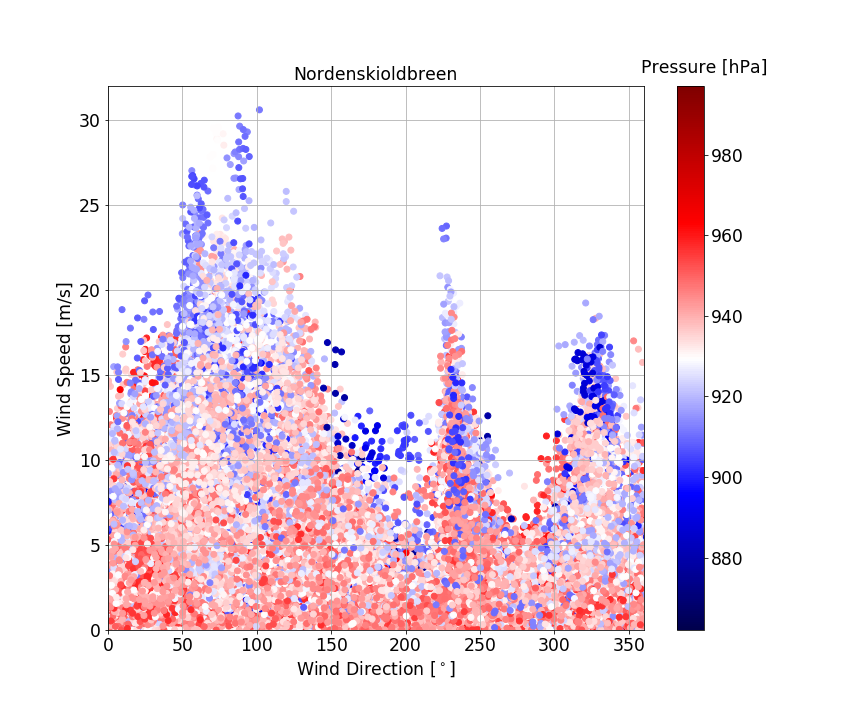
\includegraphics[scale=1, width=0.5\textwidth]{WD-WS-PR-Nordenskioldbreen.png}
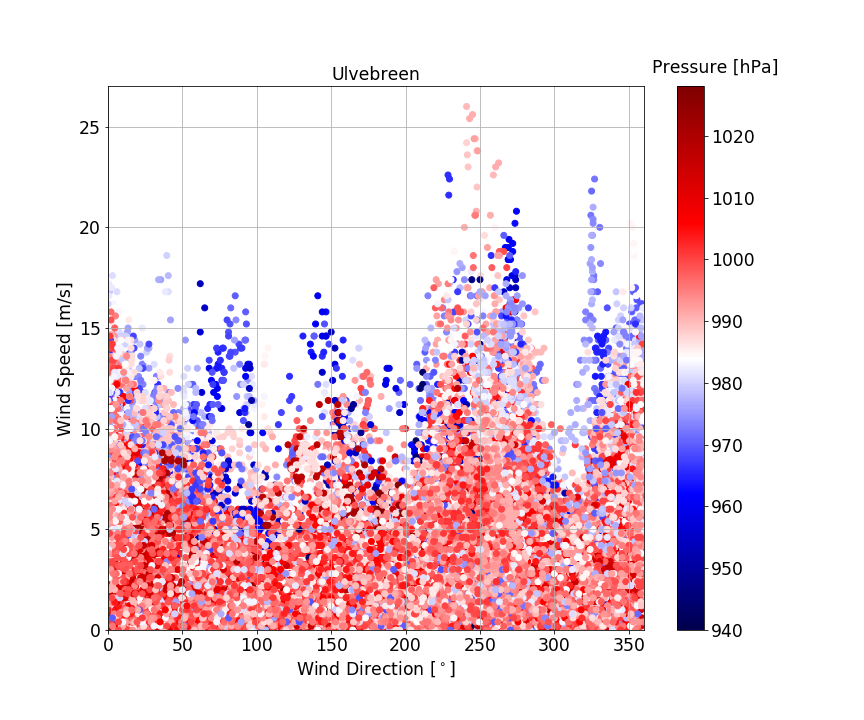
\includegraphics[scale=1, width=0.5\textwidth]{WD-WS-PR-Ulvebreen.png}
\caption{Comparison of the wind direction at x-axis, wind speed at y-axis and the corresponding pressure, related to the colourbar (all data). Measurements every 30 minutes. Left: Nordenski\H{o}ldbreen and right: Ulvebreen.}
\label{fig:PR}
\end{figure}

\newpage
Remarkable wind directions and wind speeds refer to coloured arrows. In red, the arrow for both figures corresponds to the katabatic wind, where wind is blowing down glacier corresponding to higher wind speeds and a positive difference between T2m and Tsurf. A higher T2m than Tsurf is caused by radiative cooling at the surface. The air cools, resulting in a higher density and being dragged down the slope of the glacier by gravity. This is called the katabatic wind. At the right side in figures \ref{fig:PRnorde} and \ref{fig:PRulve}, a map is plotted for both glaciers with the location of the weather station. The coloured arrows correspond with the directions of the coloured arrows in the graph on the left. 

\begin{figure}[H]
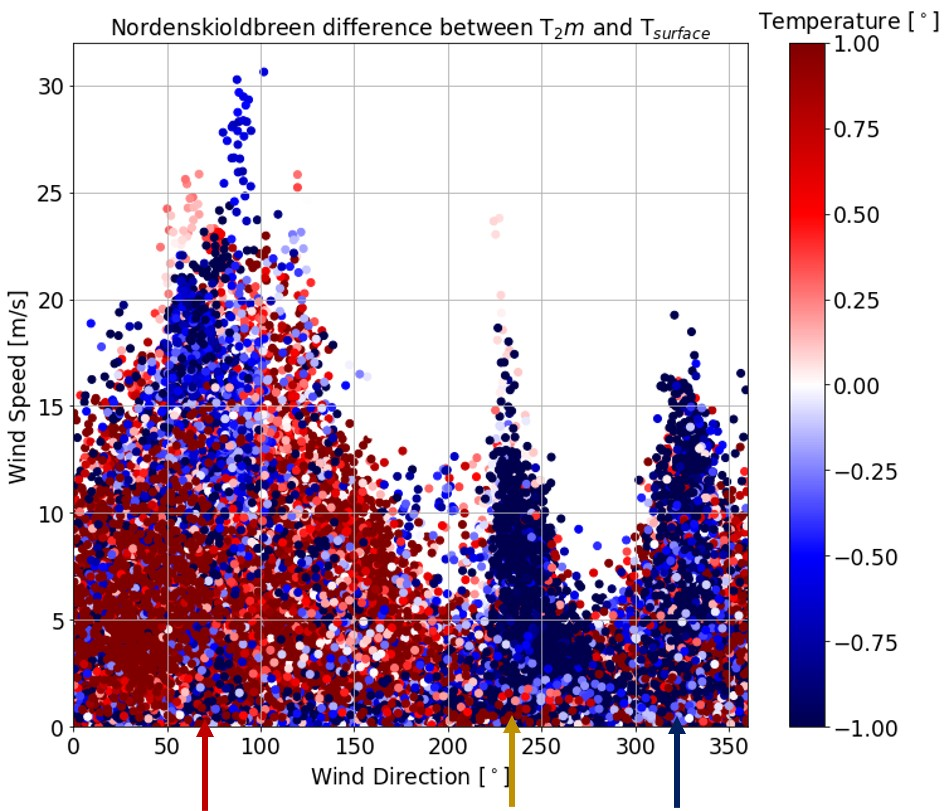
\includegraphics[scale=1, width=0.55\textwidth]{ulve-WS-WD.jpg}
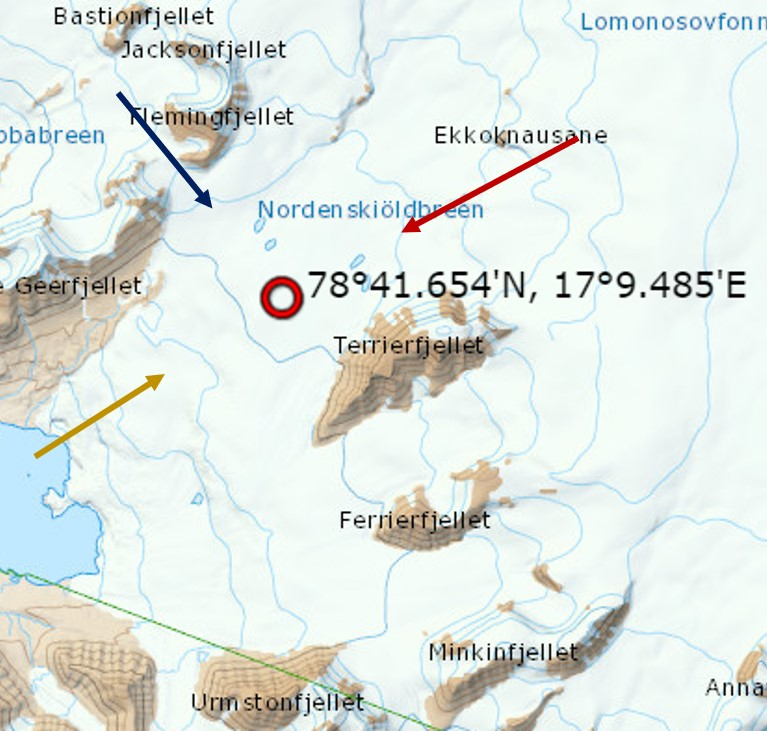
\includegraphics[scale=1, width=0.45\textwidth]{norde-WS-WD-rose-2.jpg}
\caption{Left: Comparison for the Nordenski\H{o}ldbreen of the wind direction at the x-axis, wind speed at the y-axis and the corresponding temperature, related to the colour bar (all data). In red temperature at two meter is higher than the surface temperature, conversely in blue. Right: Map \cite{NPI} of the glacier with the location of the weather station. Arrows are corresponding with the direction of the wind in the arrow on the left figure.}
\label{fig:PRnorde}
\end{figure}

\newpage
In figure \ref{fig:PRnorde} there are three wind directions that show higher wind speeds. The first one, the red arrow at 60 degrees has been discussed and is caused by the katabatic wind blowing down glacier. A second peak is visible at 240 degrees. As can be seen in the map, this wind is blowing from the bay. This wind is caused by a wind blowing through the fjord, then being pushed into the narrower bay and onto the glacier. A third peak is found at 320 degrees. This is from a wind blowing through a saddle between two mountaintops at the north west of the weather station. It can be seen that the peak at 60 degrees is much broader than the other two peaks. This is caused by the fact that the glacier, and the icecap it is flowing from, are wide. This makes the wind blow from slightly different directions. 

\begin{figure}[H]
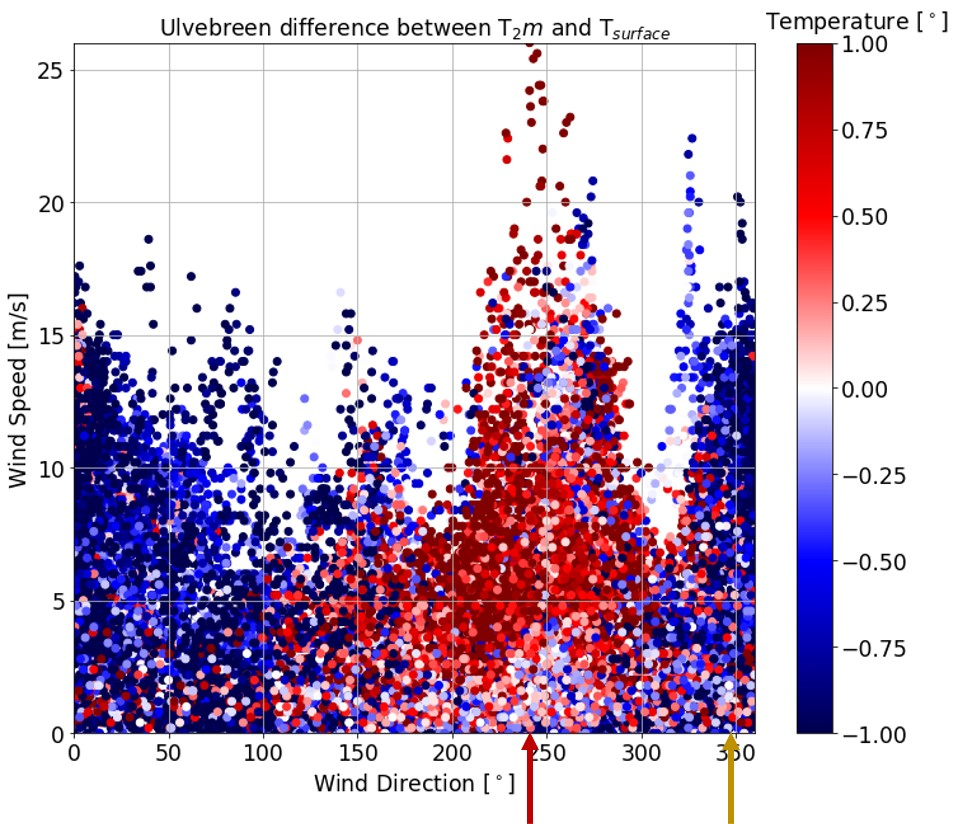
\includegraphics[scale=1, width=0.6\textwidth]{norde-WS-WD.jpg}
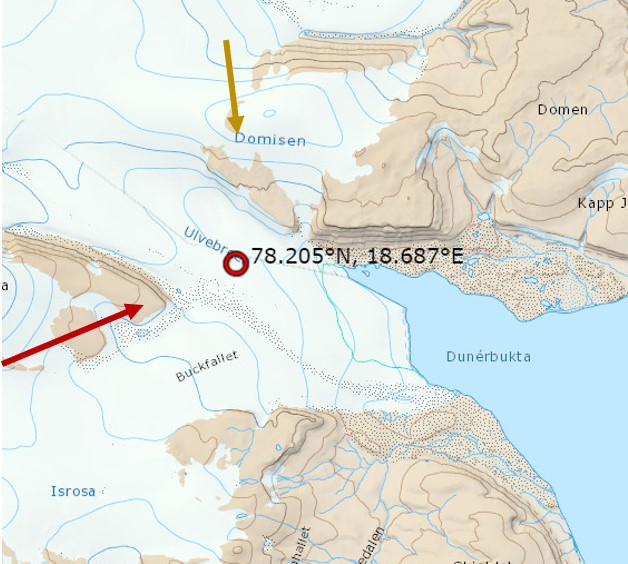
\includegraphics[scale=1, width=0.40\textwidth]{ulve-WS-WD-rose-1.jpg}
\caption{Left: Comparison for the Ulvebreen of the wind direction at x-axis, wind speed at y-axis and the corresponding temperature, related to the colourbar (all data). In red temperature at two meter is higher than the surface temperature, conversely in blue. Right: Map \cite{NPI} with wind directions, related to the coloured arrows.}
\label{fig:PRulve}
\end{figure}

We now take a look at the prevailing wind directions at the Ulvebreen (figure \ref{fig:PRulve}). We can see the katabatic peak at 250 degrees as discussed before. However, if we look at the map, this wind is coming from a cliff in the southwest. A second peak is visible at 350 degrees. This wind is blowing from another hill, north of the weather station. The wind directions are not corresponding with the expectations we had based on physics. This is further discussed in chapter \ref{sec:pw}. \\


\section{Snow and albedo}\label{sec:rad}
In this section, the relation between snow height and albedo of the Nordenski\H{o}ldbreen and the Ulvebreen are studied. First, a plot is made of the daily average values of albedo and snow surface height at the overlapping dates of the Nordenski\H{o}ldbreen and the Ulvebreen, as shown in figure \ref{fig:S1}. In this case, the snow surface height is called uncorrected, because shown are the raw data related to the distance from the sensor above the surface to the snow surface. This means that low values are a small distance between the sensor and the surface, corresponding to a high snow surface.

The data in figure \ref{fig:S1} start in autumn. It can be seen that at the beginning the albedo of the Nordenski\H{o}ldbreen is higher than the albedo of the Ulvebreen. An explanation of this could be that there already has been snowfall on the Nordenski\H{o}ldbreen and not on the Ulvebreen, which means increasing the albedo from a lower value for ice to a higher value for fresh snow. Through time, there are snow showers visible through winter, increasing the snow surface height. We can see a snowfall event at 15-10-2015 affecting both glaciers. Also, there are more local snowfall event affecting only one of the glaciers, like the event on 30-11-2015 on the Ulvebreen or on 1-1-2016 at the Nordenski\H{o}ldbreen. At the right of the graph it can be seen that summer starts again and the snow starts to melt. This happens faster at Ulvebreen than at Nordenski\H{o}ldbreen, because it its height above sea level is lower. 
Unfortunately, the overlap in data is not long enough to cover a full seasonal cycle. To investigate the whole cycle, the data is examined for each glacier apart. 

\begin{figure}[h]
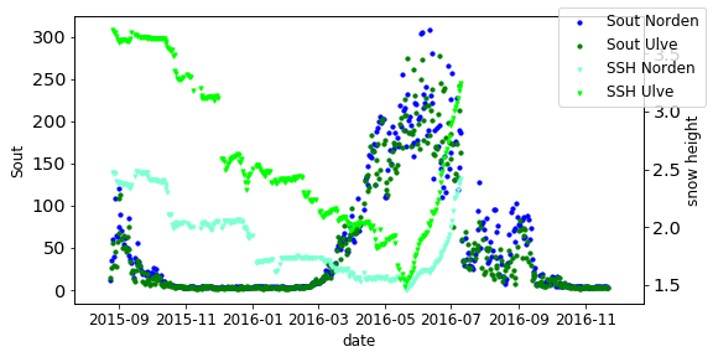
\includegraphics[scale=1, width=1\textwidth]{Picture1.jpg}
\caption{Snow surface height (``Uncorrected", see text) corresponding to the triangles and albedo corresponding to the dots, as visible in the legend for both glaciers, Nordenski\H{o}ldbreen and Ulvebreen at the overlapping dates (daily averages).}
\label{fig:S1}
\end{figure}

\begin{figure}[h]
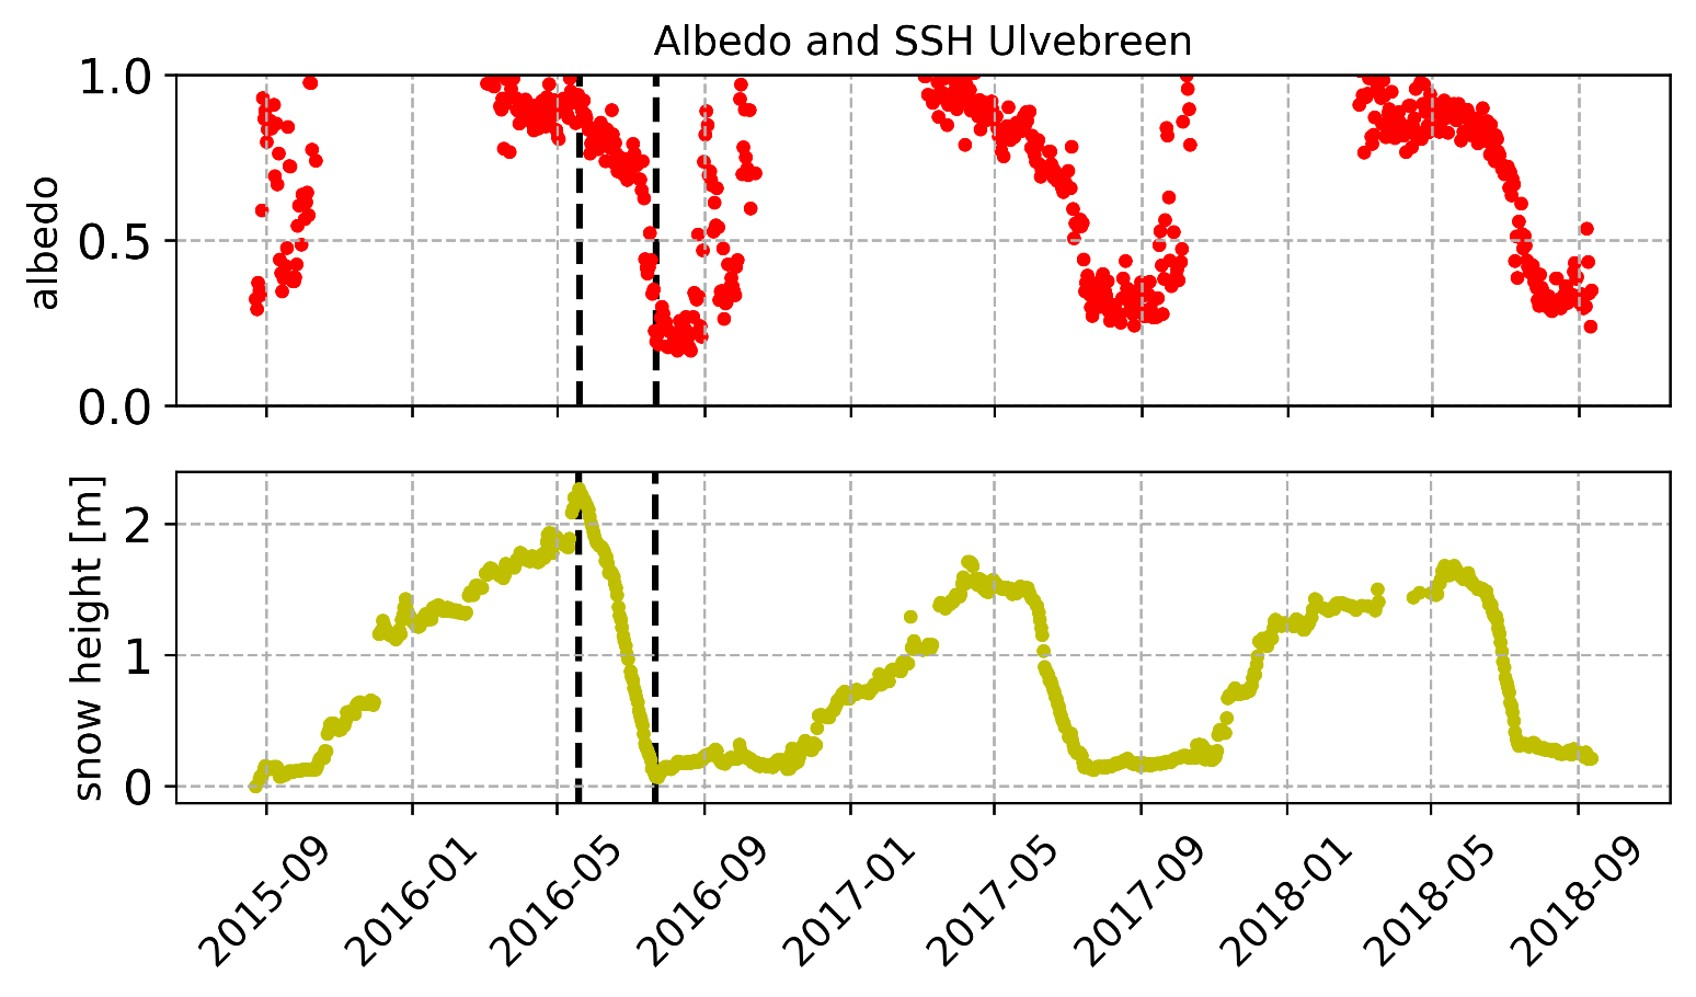
\includegraphics[scale=1, width=1\textwidth]{Picture2.jpg}
\caption{Above: Snow surface (``corrected", see text) height and below: albedo calculated for each day (daily averages) for the Ulvebreen.}
\label{fig:S2}
\end{figure}

The albedo and snow height are compared for the Ulvebreen, visible in figure \ref{fig:S2}. In this case, the snow height is `corrected'. This means the largest value of the uncorrected snow height is set to zero and from there on, the snow height compared to this level is calculated. In the beginning, when snow showers occur, the albedo increases rapidly. At the first black dotted line, after May 2016, the melt starts. There is an immediate decrease in albedo observed. This is caused by the melting of fresh snow, because wet snow has a lower albedo than fresh snow. At the second black dotted line, the snow surface height decrease stops, meaning the surface of the ice is reached. The albedo quickly drops, because ice has a lower albedo than snow. During summer, a few snow fall events happen, slightly increasing the snow height, but big increases in albedo. These thin snow layers are then quickly melted away. At the end of summer there are again increases is snowfall. This seasonal cycle is roughly repeating itself at the Ulvebreen between 2015 and 2018. 

\newpage
Furthermore, the albedo and snow height are compared for the Nordenski\H{o}ldbreen, visible in figure \ref{fig:S3}. Again, the snow height is ``corrected". The correlation between albedo and snow height is roughly the same as at the Ulvebreen. Again, through a winter season, when snow showers occur, the albedo increases rapidly. Then, at the first black dotted line around June of 2014, the process of melting starts. Like the Ulvebreen, there is an immediate decrease in albedo observed. The moment that the surface of the ice is reached is not clear in this figure, because of the different type of installation of the sensor as will be discussed in section \ref{sec:sa}. Again like the Ulvebreen, during summer, a few snow fall events happen. The second black dotted line refers to the moment that the melt stops at the start of winter. At the Nordenski\H{o}ldbreen it is harder to see the repeating process of the seasonal cycle between 2009 and 2016 as further explained in the discussion (section \ref{sec:sa}).

Also, the albedo was compared for both glaciers. In figure \ref{fig:albedo}, the albedo is shown for the overlapping period. In winter, the albedo for both glaciers is similar. However, in summer it can be seen that the albedo of the Nordenski\H{o}ldbreen is slightly higher than the albedo of the Ulvebreen. The average summer albedo over the entire measurement period for the Nordenski\H{o}ldbreen was found to be 0.53. The summer albedo was defined as the albedo during the snowfree period. The average summer albedo for the Ulvebreen was 0.44. This could be caused by a difference in ice colour, so the Nordenski\H{o}ldbreen might have cleaner and thus more reflective ice than the Ulvebreen. 

\begin{figure}[h]
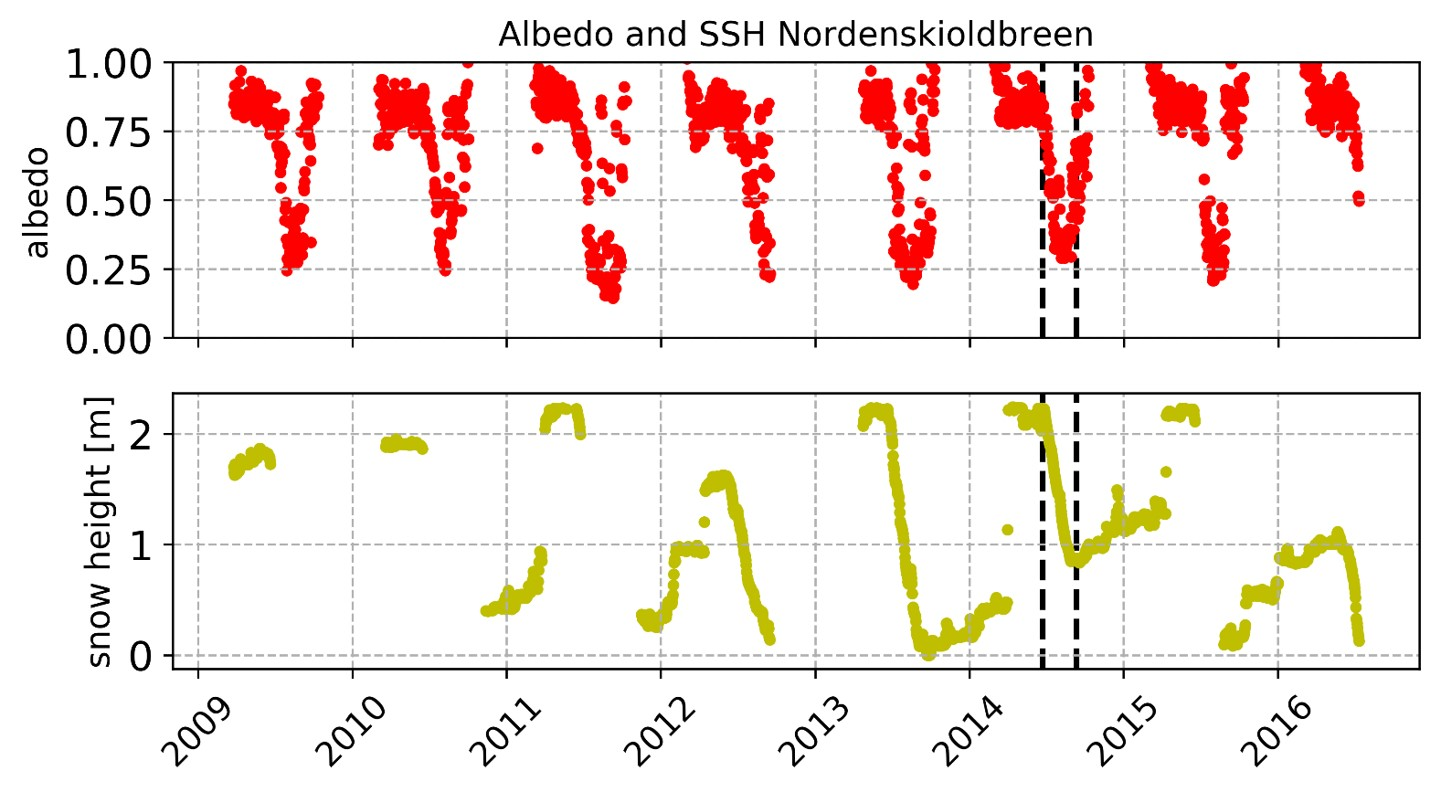
\includegraphics[scale=1, width=1\textwidth]{Picture3.jpg}
\caption{Above: Snow surface (``corrected", see text) height and below: albedo calculated for each day (daily averages) for the Nordenski\H{o}ldbreen.}
\label{fig:S3}
\end{figure}

\begin{figure}[h]
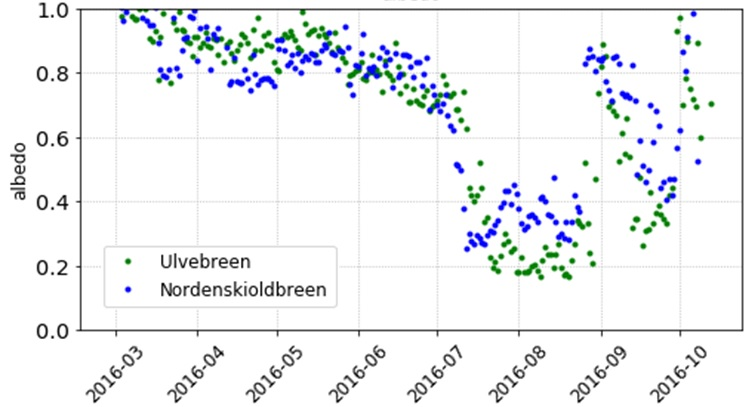
\includegraphics[scale=1, width=1 \textwidth]{albedo.jpg}
\caption{Albedo for both glaciers during the overlapping data period (daily averages).}
\label{fig:albedo}
\end{figure}


\chapter{Discussion} \label{sec:discussion}

In this chapter, results of this research are discussed. Again, this is divided in three subcategories; Temperature, Prevailing winds and Snow \& albedo, described in sections \ref{sec:Tdisc}, \ref{sec:pw} and \ref{sec:sa}, respectively. 

\section{Temperature} \label{sec:Tdisc}

The daily average temperature was calculated for all three weather stations. 30 minute data was available for the weather stations on the two glaciers, 6 hourly data was available for Svalbard Lufthavn. This could have an effect on the daily averages, meaning that the daily averages from Svalbard Lufthavn could be less accurate than for the two glaciers. However, we have set a threshold for a minimum amount of data for which we calculate the daily average. It is possible that small weather events on a timescale of less than 6 hours are now missed in the data. However, as our study looks at trends on longer timescales, this is not affecting our results a lot.

\begin{wrapfigure}{R}{0.6\textwidth}
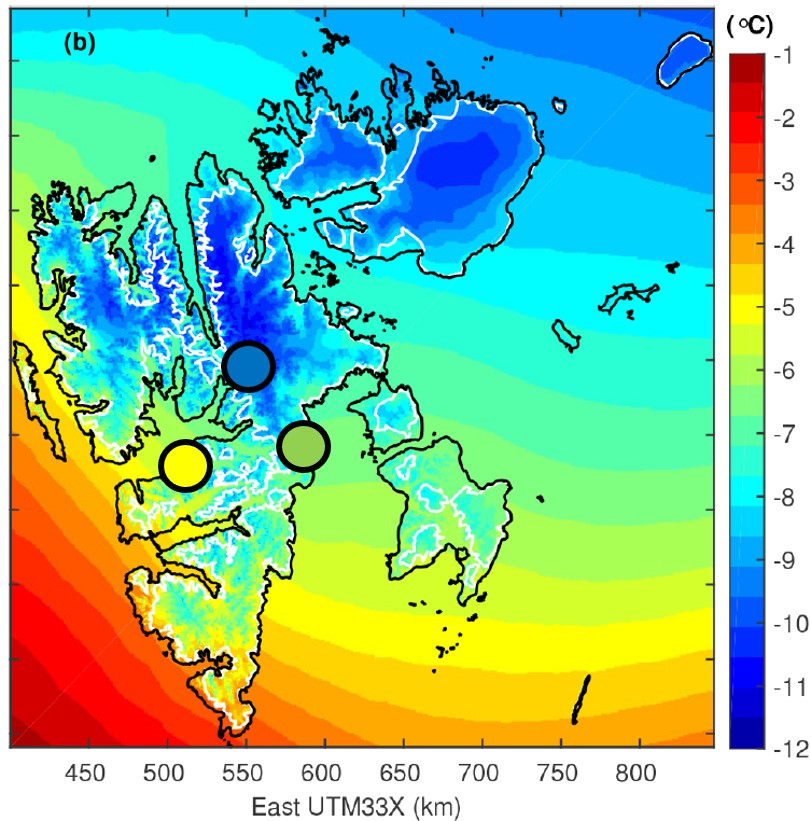
\includegraphics[width=0.6\textwidth]{ostby.jpg}
\caption{Annual mean air temperature at 2 meter averaged over 1979 to 2014 from ERA-Interim \cite{osby}}
\label{fig:trossby}
\end{wrapfigure}
The daily average temperatures for the three different locations were compared. It was found that the two glaciers do not have a significantly different temperature after correcting for the height difference. However, Svalbard Lufthavn is significantly warmer than the two glaciers. This is caused by a combination of three factors. The first is that the albedo of a glacier (ice or snow) is higher than the albedo of land (grass, water and snow around Lufthavn). The higher albedo causes more reflection and lower mean temperatures. The second cause is that in summer, the surface temperatures of a glacier do not rise above $\SI{0}{^\circ C}$, because heat energy above this will be used for glacier melt. Because the air is warmed by the surface, this results in the 2 meter temperature also not reaching far above $\SI{0}{^\circ C}$, which can be seen in figure \ref{fig:T2m} after 2016-06. This gives a large difference in 2 meter temperatures between glacier and land during summer. 

Thirdly, the location of Svalbard Lufthavn is more in the warmer south-west of the island compared to the two glacier locations. A study \cite{osby} was done that looked at the temperatures at 2 meter on Svalbard (figure \ref{fig:trossby}). In this figure, the temperature is decreasing northward as expected, but also decreasing eastward. This is caused by the higher temperatures at the west of the archipelago due to heat coming from the ocean currents. Also shown in figure \ref{fig:trossby} are the yellow, blue and green dots related to the location of the Lufthavn, Nordenski\H{o}ldbreen and Ulvebreen respectively. Since the Lufthavn is located more to the west, within the yellow temperature ``band" of $\SI{-5.5}{^\circ C}$, it seems like the Lufthavn is also warmer because of the ocean currents warming this side of the archipelago. The Nordenski\H{o}ldbreen and the Ulvebreen are in the same temperature ``band". This could explain the fact that they do not significantly differ in temperature after correcting for the height.

Another point of interest in the temperatures was shown in figure \ref{fig:Tsurf}. It could be seen that the surface temperatures on the glaciers increased above $\SI{0}{^\circ C}$. This was not expected because the surface temperature of a glacier can not heat above $\SI{0}{^\circ C}$. We have found that a high temperature is related to a high amount of shortwave radiation and low wind speeds. From this we can say that maybe the sensors are warming because of high solar radiation. Because the wind speeds are low, the sensors are not blown through to cool, and heat up, making them record higher temperatures than the surface itself has. What also needs to be kept in mind is that the sensor is placed a bit above the surface. There is a small layer of air between the surface and the sensor. This might also affect the results. 

It could also be seen that the Nordenski\H{o}ldbreen had slightly higher values above $\SI{0}{^\circ C}$ for the surface temperature than the Ulvebreen. An explanation could be that the sensor at the Nordenski\H{o}ldbreen was warmed more than the sensor at the Ulvebreen. Found was that the summer albedo for the Nordenski\H{o}ldbreen was higher than the summer albedo for the Ulvebreen. Therefore, more sunlight is reflected and may warm the sensor from beneath.\\

\section{Prevailing winds}\label{sec:pw}
Second part of the research was the prevailing winds at both glaciers. It was found that there were peaks of wind speed coming from different directions. At the Nordenski\H{o}ldbreen, we find a katabatic wind blowing down glacier, a wind blowing up from the bay and a wind blowing through a saddle between two mountain tops (figure \ref{fig:PRnorde}). 

In contrast to this, the results of the Ulvebreen do not overlap with physical expectations. We see both winds blowing from mountains, which is not what we expected. A wind was expected to blow down glacier, maybe a wind blowing from the bay upglacier and a wind from the tributary glacier Buckfallet. A possible explanation for this is that the weather station might not be installed correctly. It could be the case that the wind vane is not pointing exactly to the north. If the results are turned 15 degrees anticlockwise, it can be seen that the prevailing wind directions are now through the main glacier and the tributary glacier (figure \ref{fig:trose15}). Another unlikely but not excluded option is that the installation team used a magnetic compass. Since Svalbard is located at a latitude of roughly 78 degrees, the difference between the true North and Magnetic North can be also around 15 degrees anticlockwise (dependent on date).

A could be seen in figure \ref{fig:PR}, the high wind speeds are caused by low pressure systems passing by the island. These are thus caused by larger systems, and not by local effects. Differences between the two glaciers are mostly seen in prevailing wind directions. These are caused by the local topography, steering the wind in specific directions.

\begin{figure}[H]
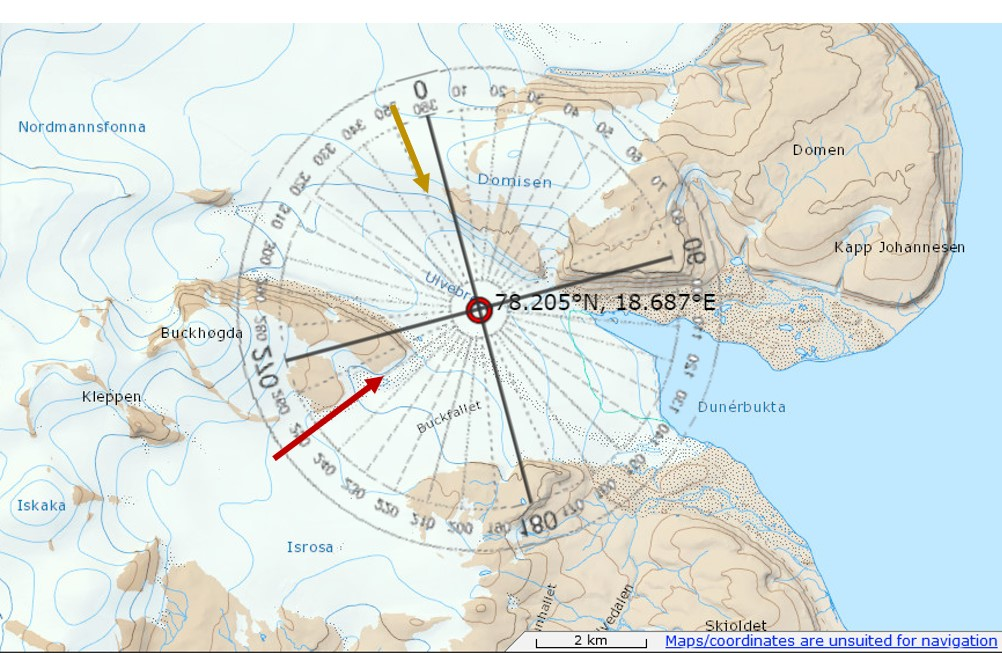
\includegraphics[scale=1, width=0.8\textwidth]{ulve-WS-WD-rose-15.jpg}
\caption{Map \cite{NPI} with wind directions, corresponding to the coloured arrows in figure \ref{fig:PRulve}. In this case, the protractor is turned 15 degrees anticlockwise.}
\label{fig:trose15}
\end{figure}


\section{Snow and albedo}\label{sec:sa}
By comparison of the snow height and albedo, it has to be taken into account that the snow height sensor of the Nordenski\H{o}ldbreen works differently than the one on the Ulvebreen. The snow height sensor at the Nordenski\H{o}ldbreen is drilled into the ice, so changes in height are because of differences in both snow and ice thickness together. This is different than the snow height sensor on the Ulvebreen, which stands on top of the ice, so changes are only caused by differences in snow thickness. A lot of gaps are visible in the measurements of snow height at the Nordenski\H{o}ldbreen (figure \ref{fig:S3}). This is caused by the fact that the weather station has had some problems in the beginning, with two periods where no data is saved. Also, the ultrasonic snow height sensor uses sound waves to determine the snow height. The speed of sound is dependent on temperature and humidity. Therefore, there are no results if the humidity and temperature sensors do not work, or if the ultrasonic sensor itself does not work. Measurements of snow height at the Nordenski\H{o}ldbreen are therefore not continuous and thus, just one stable summer period is recorded. This summer was found in 2014, visible in figure \ref{fig:S3}.

Various snowfall events were identified in figure \ref{fig:S1}. Some snowfall events affected both glaciers. These were big snowfall events passing the island. However, there were also snowfall events that only affected one of the glaciers. This has to do with the fact that the two glaciers are geographically separated by a mountain range. Some snowfall events come from the west, snow on the Nordenski\H{o}ldbreen and do not pass this mountain range. Some snowfall events come from the east, snow on the Ulvebreen and then do not pass the mountain range to the Nordenski\H{o}ldbreen. 

Another difference between the two glaciers was found in the summer albedo. The summer albedo of the Nordenski\H{o}ldbreen was higher than the summer albedo of the Ulvebreen. This is probably caused by cleaner ice at the Nordenski\H{o}ldbreen than at the Ulvebreen. 


\chapter{Conclusion}\label{sec:conclusion}

This project investigated the measurement data obtained from three weather stations in Svalbard. In this chapter the conclusions 
are drawn by answering the research questions:

\textit{What are the characteristics of the Nordenski\H{o}ldbreen and the Ulvebreen?}

The Nordenski\H{o}ldbreen is a marine terminating glacier located at 529 m a.s.l. It is located on a tributary of the Isfjord. It is therefore affected by the ocean currents that warm the west of the island. The Ulvebreen is also a marine terminating glacier. This glacier is situated at 140 m a.s.l. The Ulvebreen is situated at the east of the island Spitsbergen. Moreover, the Ulvebreen is located at a slightly lower latitude than the Nordenski\H{o}ldbreen. The distance between the two glaciers is $\SI{65}{km}$ as the crow flies. \\

\textit{What are the differences between the two glaciers?}

The first difference between the two glaciers is the mean temperature found over the overlapping data period. The mean temperature for the Nordenski\H{o}ldbreen was $\SI{-7.0}{^\circ C}$ and for the Ulvebreen $\SI{-4.9}{^\circ C}$. After the temperature was corrected for the height, the leftover difference in temperature was not significant. So the Nordenski\H{o}ldbreen is only colder than the Ulvebreen due to height differences. Taking a look at the difference in temperature between the glaciers and Svalbard Lufthavn, it was found that after correcting for height the Svalbard Lufthavn is significantly warmer than the two glaciers. 

A second difference was found in the wind directions. The highest wind speeds were caused by low pressure systems that most likely influence the whole region. The prevailing wind directions for both glaciers were different and caused by local topography.

A third difference between the two glaciers occured for snowfall events. Some snowfall events are large scale and affect both glaciers. Some are on a small scale and only have effects on one of the two. Moreover, a difference in albedo was found for the glaciers. The summer albedo of the Nordenski\H{o}ldbreen is slightly higher than the summer albedo of the Ulvebreen. This is most likely caused by a difference in the colour of the ice due to a higher sediment content in the ice of the Ulvebreen.\\

\newpage
Those answers to the sub-questions lead to an answer at the main question:

\textbf{\textit{How can the local conditions on two Svalbard glaciers be explained?}}

The main difference between the two glaciers can be explained by their difference in height above sea level. The Nordenski\H{o}ldbreen is $\SI{389}{m}$ higher than the Ulvebreen. This causes the Nordenski\H{o}ldbreen to be colder than the Ulvebreen. If corrected for height the difference in temperature between the two glaciers is not significant anymore because they are positioned in the same temperature ``band" (figure \ref{fig:trossby}). 
A difference caused by local topography are the prevailing wind directions. Moreover, the difference in snowfall events is caused by the different location on the island. However, there are also large atmospheric circulation patterns affecting both glaciers, as can be seen from the fact that the highest wind speeds are found for low pressure events and the big snowfall events that affect both glaciers.  \\

While doing research on the data from weather stations, it needs to be kept in mind that there are some measurement uncertainties. Clear measurement uncertainties found in this study were the found prevailing wind directions on the Ulvebreen, which might have been caused by a mistake in the installation of the weather station, and the surface temperatures that reach values above $\SI{0}{^\circ C}$. 
To get a better understanding of the effects of climate change on the glaciers in Svalbard, a good understanding of the local conditions is necessary. Due to the uncertainties and the low availability of long time series, it is important to further study the characteristics and weather conditions on glaciers in the Arctic.

\begin{thebibliography}{9}
\addcontentsline{toc}{chapter}{Bibliography}

%1
\bibitem{sval}
Website: The University Centre in Svalbard, UNIS (01-2018), 
\textit{The Early Exploration of the Arctic and the Discovery of
Svalbard},
Retrieved at 30-10-2018, from:\\
\texttt{\small{https://www.unis.no/wp-content/uploads/2018/01/SH201\_Summary02\_2018.pdf}}

%2
\bibitem{sees}
Website: Netherlands Scientific Expedition Edge{\o}ya Spitsbergen, SEES, (2015), \\ Retrieved at 30-10-2018, from:
\texttt{\small{http://www.sees.nl/}}

%3
\bibitem{1}
Website: Norwegian Meteorological Institute Svalbard climate data
\textit{Weather statistics for Longyearbyen (Svalbard)},
Retrieved at 30-10-2018, from:
\texttt{https://www.yr.no/place/Norway/Svalbard/Longyearbyen/statistics.html}

%4
\bibitem{2}
Article: Storrie, L., Lydersen, C., Andersen, M., B.Wynn, R. and Kovacs, K. (2018). 
\textit{Determining the species assemblage and habitat use of cetaceans in the Svalbard Archipelago, based on observations from 2002 to 2014.} Polar Research, \texttt{ https://doi.org/10.1080/17518369.2018.1463065} 

%5
\bibitem{NPI}
Website: Norwegian Polar Institute (NPI) 
\textit{Kart over Svalbard},\\
Retrieved at 25-09-2018, from: \texttt{https://toposvalbard.npolar.no/}

%6
\bibitem{uuproj}
Website: Institute for Marine and Atmospheric Research (IMAU)
\textit{Ice and Climate: Automatic Weather Stations on glaciers.}
Retrieved at 30-10-2018, from:
\texttt{https://www.projects.science.uu.nl/iceclimate/aws/files\_oper/}

%7
\bibitem{abl}
Article: Hulth, J. (2010). 
\textit{Using a draw-wire sensor to continuously monitor glacier melt.} Journal of Glaciology, 56(199), 922-924. 
\texttt{https://doi:10.3189/002214310794457290}

%8
\bibitem{sharkii}
Website: eKlima \textit{the climate database of the Norwegian Meteorological Institute}, Retrieved at 1-10-2018, from:
\texttt{http://sharki.oslo.dnmi.no/}

\bibitem{brzblak}
Article: Przybylak, R. , Araźny, A. , Nordli, {\O}. , Finkelnburg, R. , Kejna, M. , Budzik, T. , Migała, K. , Sikora, S. , Puczko, D. , Rymer, K. and Rachlewicz, G. (2014), \textit{Spatial distribution of air temperature on Svalbard during 1 year with campaign measurements.} Int. J. Climatol., 34: 3702-3719. \texttt{https://doi:10.1002/joc.3937}

%9
\bibitem{osby}
Article: {\O}stby, T. I., Schuler, T. V., Hagen, J. O., Hock, R., Kohler, J., and Reijmer, C. H.  (2017),: \texttt{Diagnosing the decline in climatic mass balance of glaciers in Svalbard over 1957–2014}, The Cryosphere, 11, 191-215 \texttt{https://doi.org/10.5194/tc-11-191-2017}

\end{thebibliography}

%\chapter*{Appendices}
%\addcontentsline{toc}{chapter}{Appendices}

%\section*{A. name}\label{Ap:A}
%\setcounter{figure}{0}
%\renewcommand{\thefigure}{A.\arabic{figure}}
%\addcontentsline{toc}{section}{A. name}

\end{document}
